%package list
\documentclass{article}
\usepackage[top=3cm, bottom=3cm, outer=3cm, inner=3cm]{geometry}
\usepackage{multicol}
\usepackage{graphicx}
\usepackage{url}
%\usepackage{cite}
\usepackage{hyperref}
\usepackage{array}
%\usepackage{multicol}
\newcolumntype{x}[1]{>{\centering\arraybackslash\hspace{0pt}}p{#1}}
\usepackage{natbib}
\usepackage{pdfpages}
\usepackage{multirow}
\usepackage[normalem]{ulem}
\useunder{\uline}{\ul}{}
\usepackage{svg}
\usepackage{xcolor}
\usepackage{listings}

\lstdefinestyle{ascii-tree}{
    literate={├}{|}1 {─}{--}1 {└}{+}1 
  }
\lstset{basicstyle=\ttfamily,
  showstringspaces=false,
  commentstyle=\color{red},
  keywordstyle=\color{blue}
}
%\usepackage{booktabs}
\usepackage{caption}
\usepackage{subcaption}
\usepackage{float}
\usepackage{array}

\newcolumntype{M}[1]{>{\centering\arraybackslash}m{#1}}
\newcolumntype{N}{@{}m{0pt}@{}}


%%%%%%%%%%%%%%%%%%%%%%%%%%%%%%%%%%%%%%%%%%%%%%%%%%%%%%%%%%%%%%%%%%%%%%%%%%%%
%%%%%%%%%%%%%%%%%%%%%%%%%%%%%%%%%%%%%%%%%%%%%%%%%%%%%%%%%%%%%%%%%%%%%%%%%%%%
\newcommand{\itemEmail}{kllacma@unsa.edu.pe}
\newcommand{\itemStudent}{Kevin Andree Llacma Quispe}
\newcommand{\itemCourse}{Programacion web 2}
\newcommand{\itemCourseCode}{20200585}
\newcommand{\itemSemester}{I}
\newcommand{\itemUniversity}{Universidad Nacional de San Agustín de Arequipa}
\newcommand{\itemFaculty}{Facultad de Ingeniería de Producción y Servicios}
\newcommand{\itemDepartment}{Departamento Académico de Ingeniería de Sistemas e Informática}
\newcommand{\itemSchool}{Escuela Profesional de Ingeniería de Sistemas}
\newcommand{\itemAcademic}{2024 - A}
\newcommand{\itemInput}{-}
\newcommand{\itemOutput}{-}
\newcommand{\itemPracticeNumber}{06}
\newcommand{\itemTheme}{Django(Admin)}
%%%%%%%%%%%%%%%%%%%%%%%%%%%%%%%%%%%%%%%%%%%%%%%%%%%%%%%%%%%%%%%%%%%%%%%%%%%%
%%%%%%%%%%%%%%%%%%%%%%%%%%%%%%%%%%%%%%%%%%%%%%%%%%%%%%%%%%%%%%%%%%%%%%%%%%%%

\usepackage[english,spanish]{babel}
\usepackage[utf8]{inputenc}
\AtBeginDocument{\selectlanguage{spanish}}
\renewcommand{\figurename}{Figura}
\renewcommand{\refname}{Referencias}
\renewcommand{\tablename}{Tabla} %esto no funciona cuando se usa babel
\AtBeginDocument{%
	\renewcommand\tablename{Tabla}
}

\usepackage{fancyhdr}
\pagestyle{fancy}
\fancyhf{}
\setlength{\headheight}{30pt}
\renewcommand{\headrulewidth}{1pt}
\renewcommand{\footrulewidth}{1pt}
\fancyhead[L]{\raisebox{-0.2\height}{
\includegraphics[width=3cm]{img/logo_episunsa.png}}}
\fancyhead[C]{\fontsize{7}{7}\selectfont	\itemUniversity \\ \itemFaculty \\ \itemDepartment \\ \itemSchool \\ \textbf{\itemCourse}}
\fancyhead[R]{\raisebox{-0.2\height}{
\includegraphics[width=1.2cm]{img/logo_abet}}}
\fancyfoot[L]{Estudiante Kevin Llacma}
\fancyfoot[C]{\itemCourse}
\fancyfoot[R]{Página \thepage}

% para el codigo fuente

\usepackage{listings}
\usepackage{color, colortbl}
\definecolor{dkgreen}{rgb}{0,0.6,0}
\definecolor{gray}{rgb}{0.5,0.5,0.5}
\definecolor{mauve}{rgb}{0.58,0,0.82}
\definecolor{codebackground}{rgb}{0.95, 0.95, 0.92}
\definecolor{tablebackground}{rgb}{0.8, 0, 0}

\lstset{frame=tb,
	language=bash,
	aboveskip=3mm,
	belowskip=3mm,
	showstringspaces=false,
	columns=flexible,
	basicstyle={\small\ttfamily},
	numbers=none,
	numberstyle=\tiny\color{gray},
	keywordstyle=\color{blue},
	commentstyle=\color{dkgreen},
	stringstyle=\color{mauve},
	breaklines=true,
	breakatwhitespace=true,
	tabsize=3,
	backgroundcolor= \color{codebackground},
}

\begin{document}
	
	\vspace*{10px}
	
	\begin{center}	
		\fontsize{17}{17} \textbf{ Informe de Laboratorio \itemPracticeNumber}
	\end{center}
	\centerline{\textbf{\Large Tema: \itemTheme}}
	%\vspace*{0.5cm}	

	\begin{flushright}
		\begin{tabular}{|M{2.5cm}|N|}
			\hline 
			\rowcolor{tablebackground}
			\color{white} \textbf{Nota}  \\
			\hline 
			     \\[30pt]
			\hline 			
		\end{tabular}
	\end{flushright}	

	\begin{table}[H]
		\begin{tabular}{|x{4.7cm}|x{4.8cm}|x{4.8cm}|}
			\hline 
			\rowcolor{tablebackground}
			\color{white} \textbf{Estudiante} & \color{white}\textbf{Escuela}  & \color{white}\textbf{Asignatura}   \\
			\hline 
			{\itemStudent \par \itemEmail} & \itemSchool & {\itemCourse \par Semestre: \itemSemester \par Código: \itemCourseCode}     \\
			\hline 			
		\end{tabular}
	\end{table}		
	
	\begin{table}[H]
		\begin{tabular}{|x{4.7cm}|x{4.8cm}|x{4.8cm}|}
			\hline 
			\rowcolor{tablebackground}
			\color{white}\textbf{Laboratorio} & \color{white}\textbf{Tema}  & \color{white}\textbf{Duración}   \\
			\hline 
			\itemPracticeNumber & \itemTheme & 04 horas   \\
			\hline 
		\end{tabular}
	\end{table}
	
	\begin{table}[H]
		\begin{tabular}{|x{4.7cm}|x{4.8cm}|x{4.8cm}|}
			\hline 
			\rowcolor{tablebackground}
			\color{white}\textbf{Semestre académico} & \color{white}\textbf{Fecha de inicio}  & \color{white}\textbf{Fecha de entrega}   \\
			\hline 
			\itemAcademic & \itemInput &  \itemOutput  \\
			\hline 
		\end{tabular}
	\end{table}
\title{Programación Web\\Laboratorio 06\\Tema: Django(Admin)}

\maketitle


\section{Marco teorico}


\subsection{Django}

    \begin{itemize}
        \item Django es un framework web Python con el cuál el desarrollo de sitios web son rápidos, seguros y sobre todo fáciles de mantener.
        \item Django se ocupa de gran parte de las molestias del desarrollo web, por lo que puede concentrarse en escribir su aplicación sin necesidad de reinventar la rueda.
        \item Es software libre, tiene una comunidad próspera y activa, excelente documentación y muchas opciones de soporte gratuito y de pago.
    \end{itemize}


\section{Desarollo del lab}
\subsection{Descripcion}
\textbf{Proyecto Tienda online}
\\Para empezar este proyecto se creo un entorno virtual

\\Luego se procedio a instalar django con mysqlclient para base de datos
\\A continuacion se creo un proyecto llamado "tiendaonline" y se creo la app "shop"


    \begin{figure}[H]
		          \centering
		          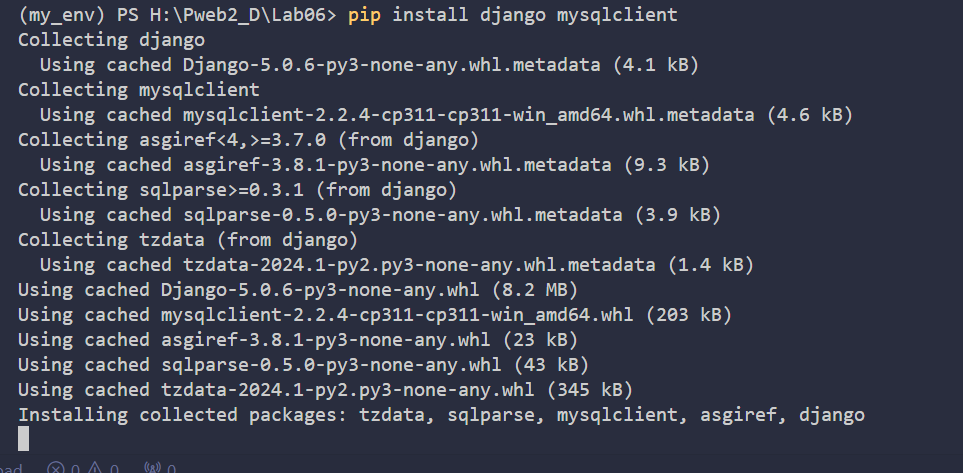
\includegraphics[width=0.8\textwidth,keepaspectratio]                       {img/djangoIns.png}
		             %\includesvg{img/automata.svg}
		              %\label{img:mot2}
		              %\caption{Product backlog.}
    \end{figure}
\\
    \begin{figure}[H]
		          \centering
		          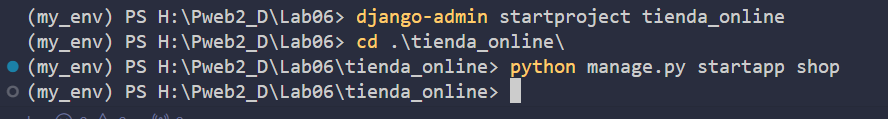
\includegraphics[width=0.8\textwidth,keepaspectratio]                       {img/iniApp.png}
		             %\includesvg{img/automata.svg}
		              %\label{img:mot2}
		              %\caption{Product backlog.}
    \end{figure}

\\    
    
Luego se configuro settings.py para la base de datos, si fuera sqlite no se tendria que identificar
    \begin{figure}[H]
		          \centering
		          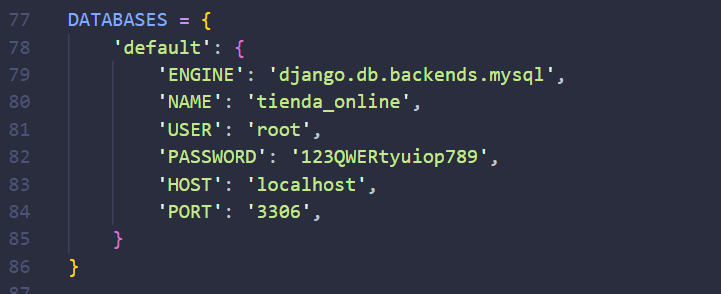
\includegraphics[width=0.8\textwidth,keepaspectratio]                       {img/settings.png}
		             %\includesvg{img/automata.svg}
		              %\label{img:mot2}
		              %\caption{Product backlog.}
    \end{figure}
\\
Ahora hacemos lo modelos tablas, en este caso que es una tienda se busco que tablas se podria agregar en un caso real (en models.py)
\\Usuario categoria y producto
\begin{itemize}
    \item A usuario le pide nombre, email, correro y contraseña
    \item categoria tiene solo nombre y descripcion
    \item Producto ademas de eso tiene un precio y un stock
\end{itemize}

     \begin{figure}[H]
		          \centering
		          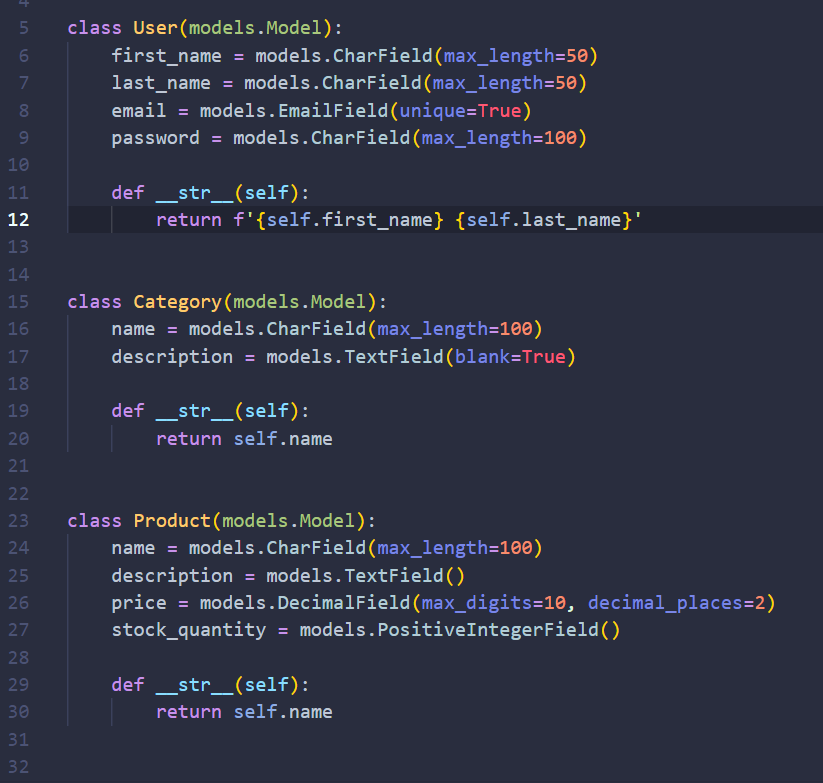
\includegraphics[width=0.8\textwidth,keepaspectratio]                       {img/UserCatPro.png}
		             %\includesvg{img/automata.svg}
		              %\label{img:mot2}
		              %\caption{Product backlog.}
    \end{figure}
\\
\\Continuamos con los siguietne modelos y explicando un poco en que consiten
ProductCategory: Relación entre productos y categorías
\begin{itemize}
    \item product: Producto relacionado
    \item category: Categoría relacionada
\end{itemize}
Order: Representa los pedidos realizados por los usuarios
\begin{itemize}
    \item user: Usuario que realizó el pedido
    \item orderdate: Fecha en la que se creó el pedido
    \item status: Estado del pedido 
\end{itemize}
OrderDetail: Detalles específicos de cada producto en un pedido.
\begin{itemize}
    \item order: Pedido al que pertenece.
    \item product: Producto del pedido.
    \item quantity: Cantidad de producto en el pedido.
    \item price: Precio del producto en el momento del pedido.
\end{itemize}
ShoppingCart: Carritos de compras de los usuarios
\begin{itemize}
    \item user: Usuario al que pertenece el carrito
    \item createdat: Fecha de creación del carrit
\end{itemize}
CartDetail: Detalles de los productos en un carrito de compas.
\begin{itemize}
    \item shoppingcart: Carrito de compras al que pertenece
    \item product: Producto en el carrito
    \item quantity: Cantidad del produto en el carrito
\end{itemize}
    \begin{figure}[H]
		          \centering
		          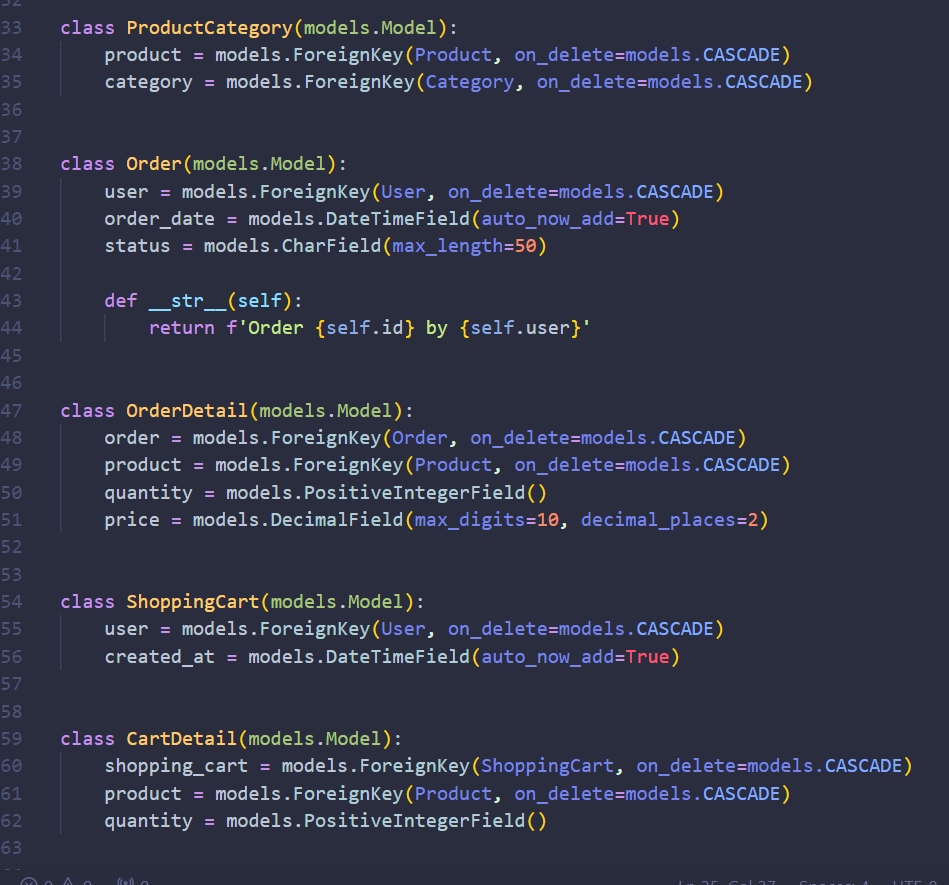
\includegraphics[width=0.8\textwidth,keepaspectratio]                       {img/PrctOrDetShoCart.png}
		             %\includesvg{img/automata.svg}
		              %\label{img:mot2}
		              %\caption{Product backlog.}
    \end{figure}
\

\\Se busco informacion para hacer los requisitos de manera real 
\\Direccion y Pago:
Address: Direcciones de los usuarios
\begin{itemize}
    \item user: Usuario al que pertenece la dirección
    \item addressline: Línea prncipal de la dirección
    \item city: Ciudad
    \item state: Estado o provncia
    \item zipcode: Codigo postal
    \item country: Pais
\end{itemize}
Payment: Pagos realizados para los pedidos
\begin{itemize}
    \item order: Pedido al que se relaciona el pago
    \item paymentdate: Fecha del pago
    \item amount: Monto pagad
    \item paymentmethod: Método de pago
\end{itemize}

    \begin{figure}[H]
		          \centering
		          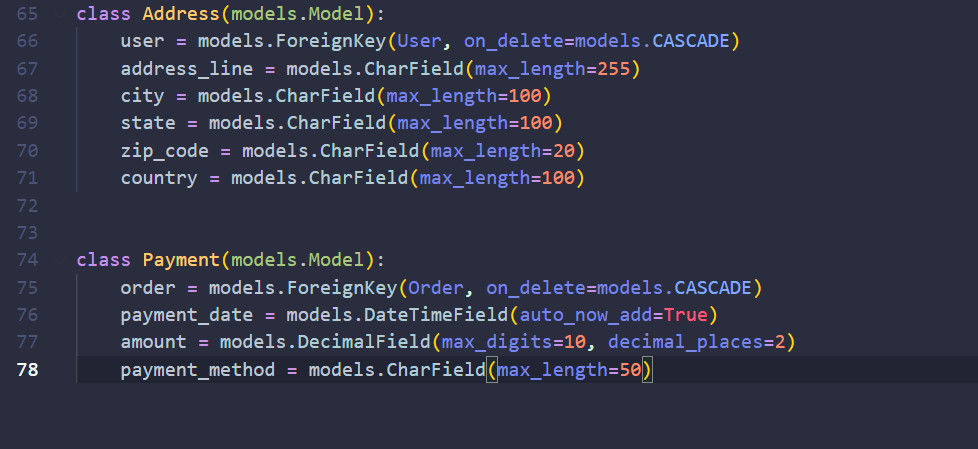
\includegraphics[width=0.8\textwidth,keepaspectratio]                       {img/AddPay.png}
		             %\includesvg{img/automata.svg}
		              %\label{img:mot2}
		              %\caption{Product backlog.}
    \end{figure}
\\Luego los registramos en Admin.py 

    \begin{figure}[H]
		          \centering
		          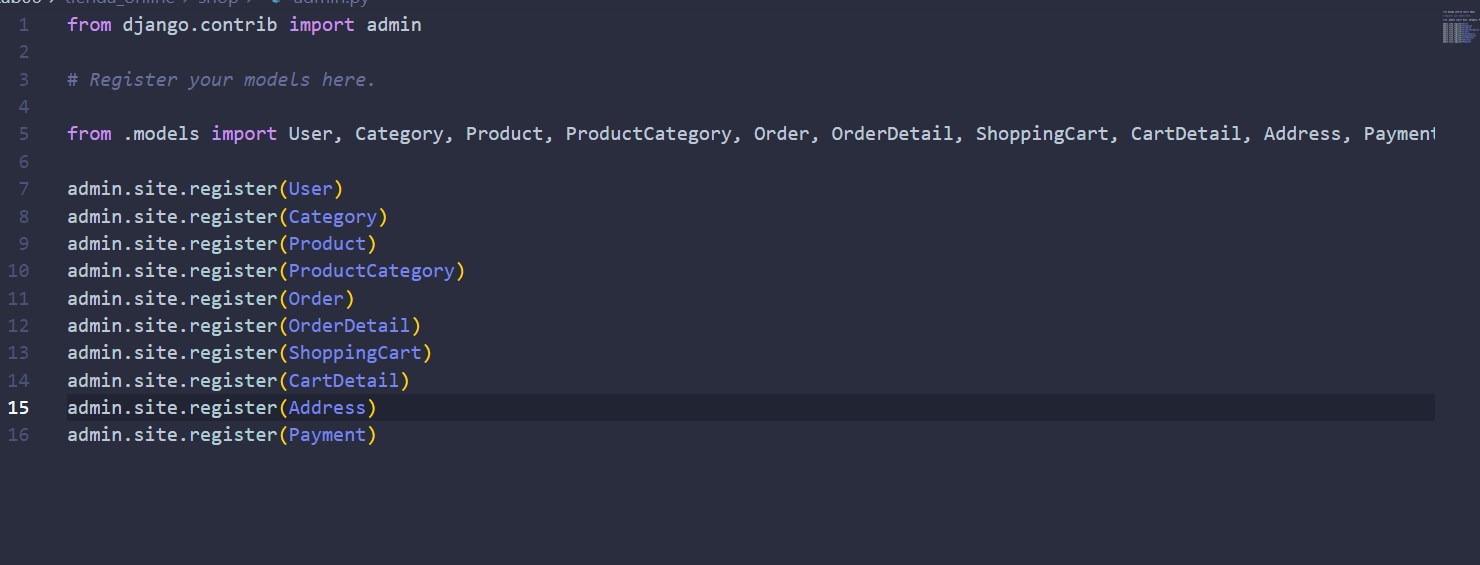
\includegraphics[width=0.8\textwidth,keepaspectratio]                       {img/register.png}
		             %\includesvg{img/automata.svg}
		              %\label{img:mot2}
		              %\caption{Product backlog.}
    \end{figure}



\\Ahora creamos y aplicamos migraciones

     \begin{figure}[H]
		          \centering
		          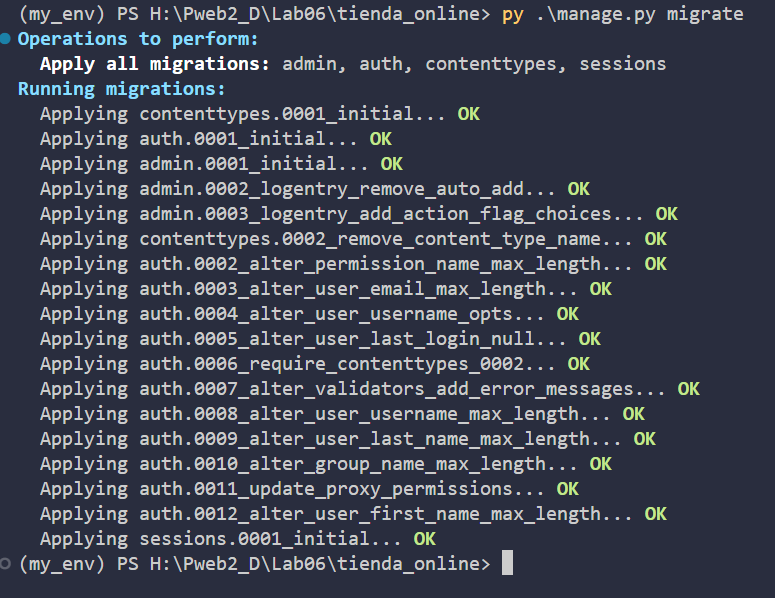
\includegraphics[width=0.8\textwidth,keepaspectratio]                       {img/migration.png}
		             %\includesvg{img/automata.svg}
		              %\label{img:mot2}
		              %\caption{Product backlog.}
    \end{figure}


\\Ahora creando un superusuario

     \begin{figure}[H]
		          \centering
		          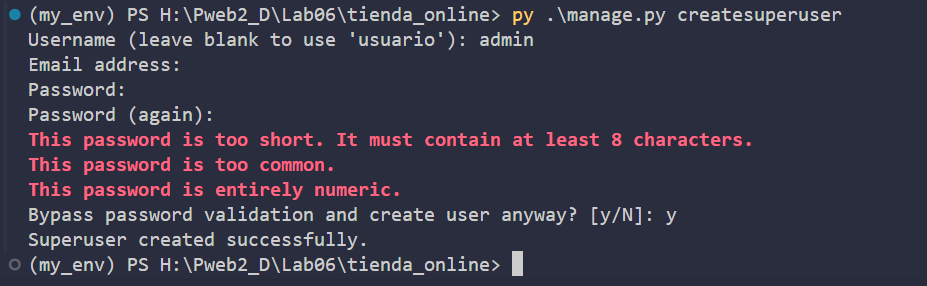
\includegraphics[width=0.8\textwidth,keepaspectratio]                       {img/admin.png}
		             %\includesvg{img/automata.svg}
		              %\label{img:mot2}
		              %\caption{Product backlog.}
    \end{figure}

\\Iniciamos el server

    \begin{figure}[H]
		          \centering
		          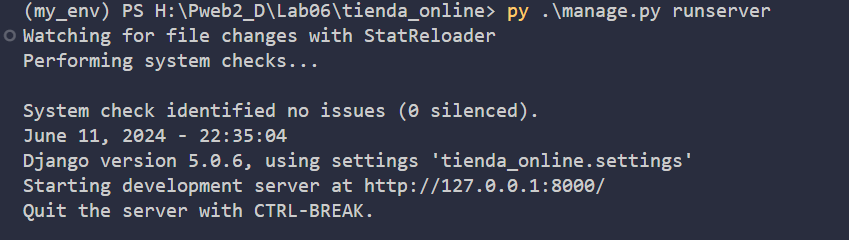
\includegraphics[width=0.8\textwidth,keepaspectratio]                       {img/runserver.png}
		             %\includesvg{img/automata.svg}
		              %\label{img:mot2}
		              %\caption{Product backlog.}
    \end{figure}
    
\\Observamos como se ve admin y accedemos con superusuario

    \begin{figure}[H]
		          \centering
		          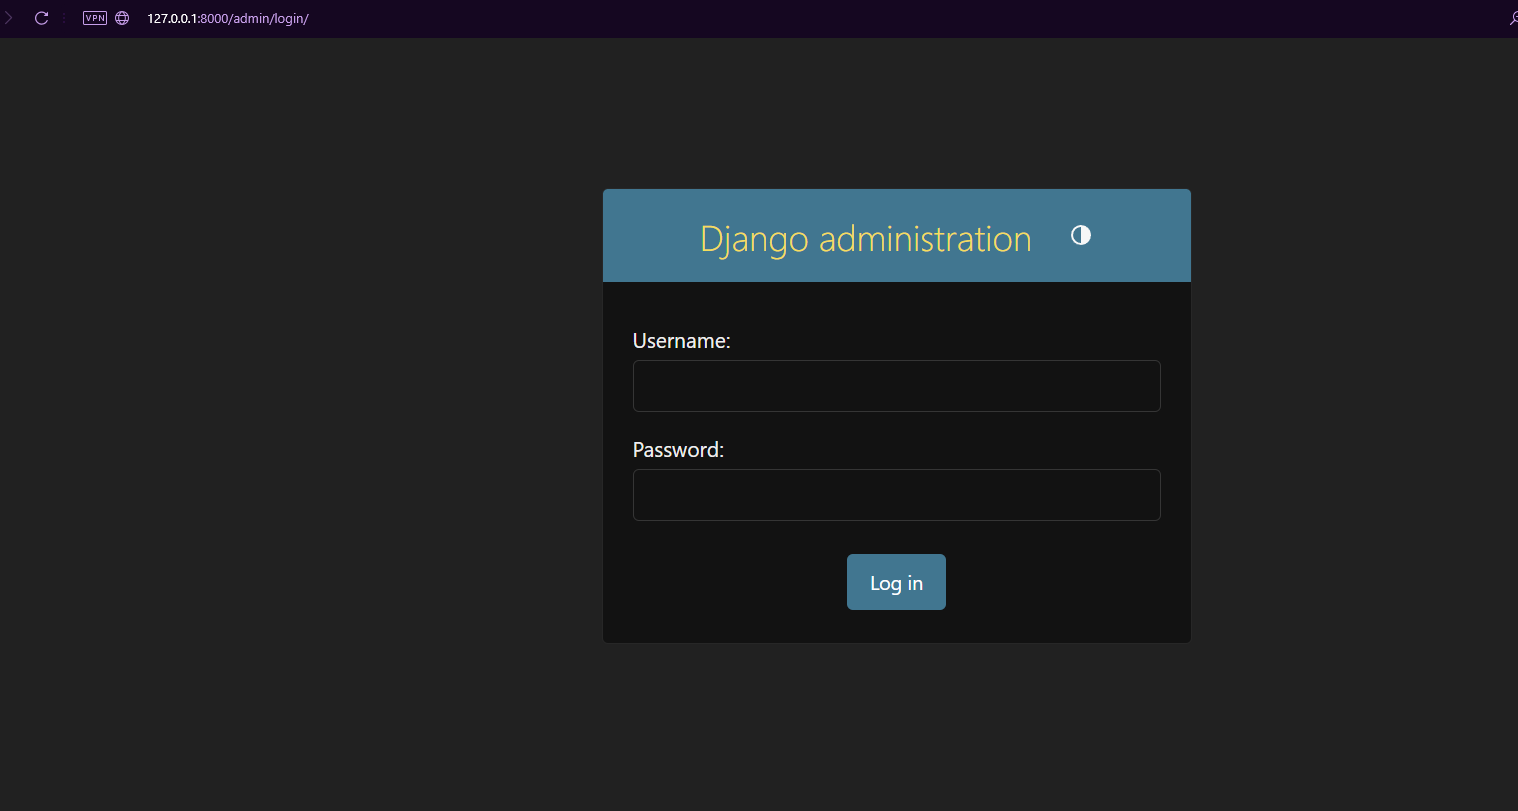
\includegraphics[width=0.8\textwidth,keepaspectratio]                       {img/login.png}
		             %\includesvg{img/automata.svg}
		              %\label{img:mot2}
		              %\caption{Product backlog.}
    \end{figure}

\\

\\Accdemos y observamos la tablas que creamos

    \begin{figure}[H]
		          \centering
		          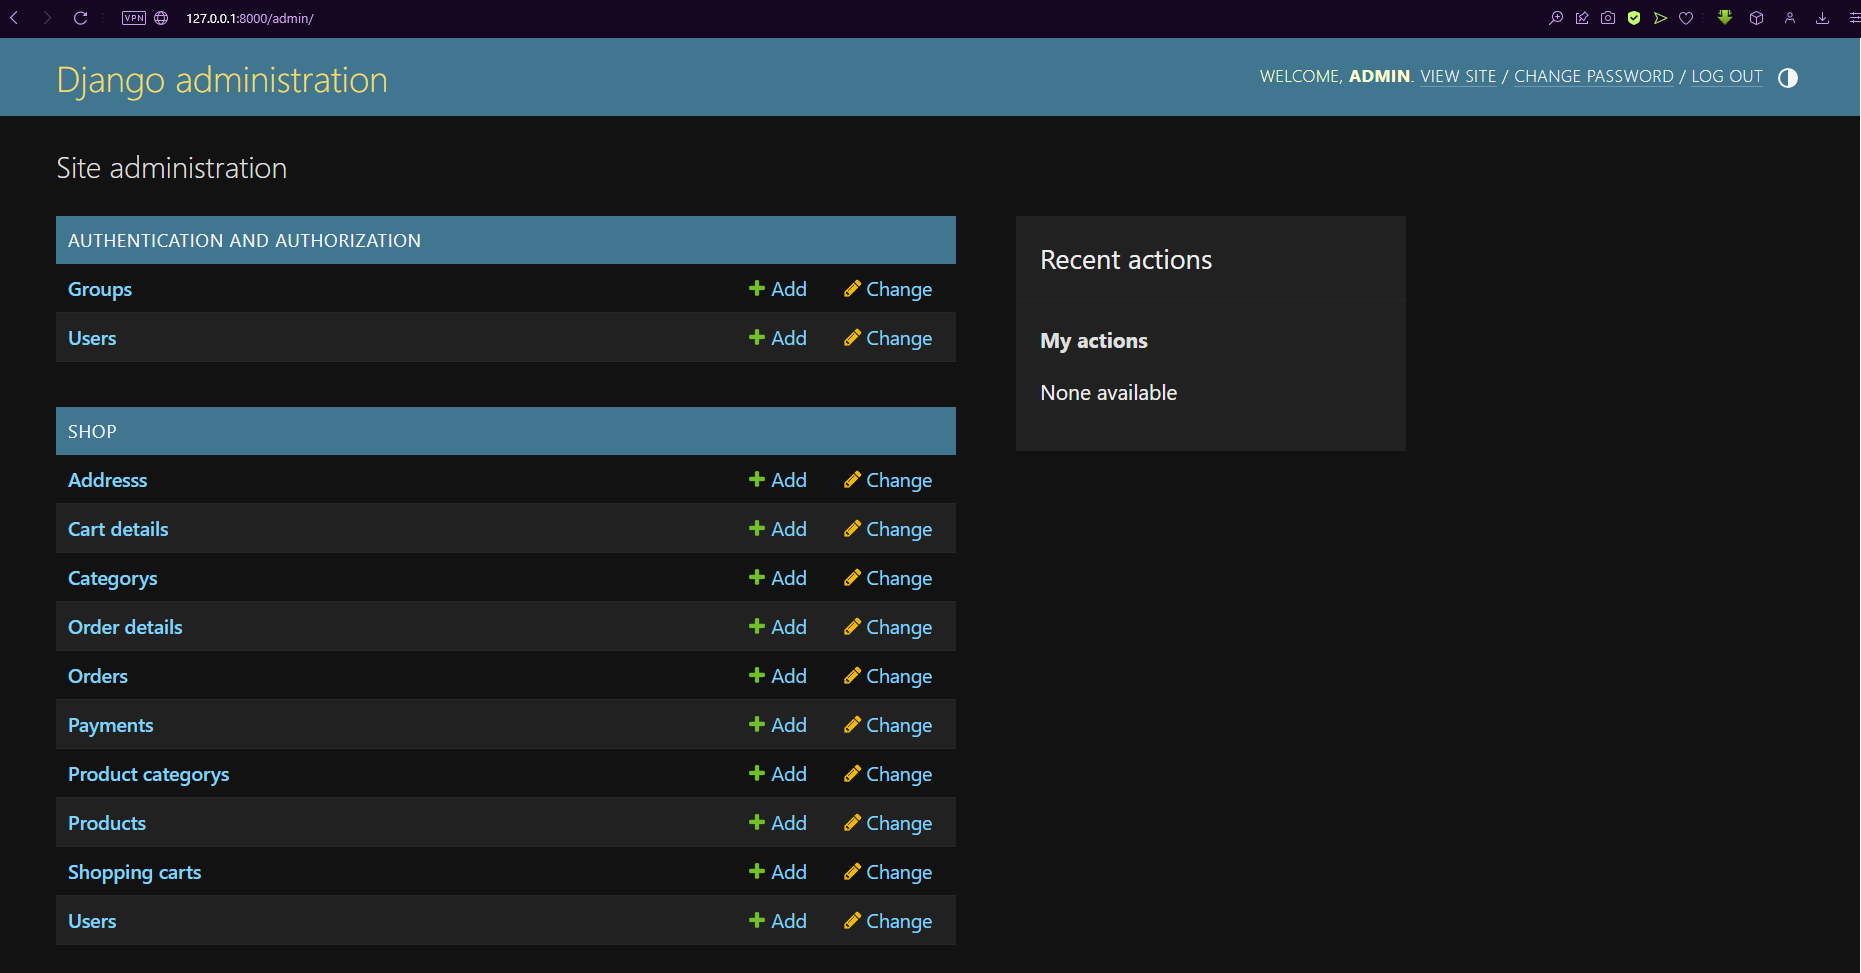
\includegraphics[width=0.8\textwidth,keepaspectratio]                       {img/djadmin.png}
		             %\includesvg{img/automata.svg}
		              %\label{img:mot2}
		              %\caption{Product backlog.}
    \end{figure}    
\\


\end{document}